\chapter{Instrumental learning}


Form of control learning that aims to learn action-outcome associations:
\begin{itemize}
    \item When a reinforcer is likely to occur.
    \item Which actions bring to those reinforcers.
\end{itemize}
This allows the animal to act in anticipation of a reinforcer.

Instrumental learning includes:
\begin{descriptionlist}
    \item[Habitual system] \marginnote{Habitual system}
        Learn to repeat previously successful actions.
    \item[Goal-directed system] \marginnote{Goal-directed system}
        Evaluate actions based on their anticipated consequences.
\end{descriptionlist}

Depending on the outcome, the effect varies:
\begin{descriptionlist}
    \item[Positive reinforcement] \marginnote{Positive reinforcement}
        Delivering an appetitive outcome to an action increases the probability of emitting it.

    \item[Positive punishment] \marginnote{Positive punishment}
        Delivering an aversive outcome to an action decreases the probability of emitting it.
    
    \item[Negative reinforcement] \marginnote{Negative reinforcement}
        Omitting an aversive outcome to an action increases the probability of emitting it.
    
    \item[Negative punishment] \marginnote{Negative punishment}
        Omitting an appetitive outcome to an action decreases the probability of emitting it.
\end{descriptionlist}

\begin{table}[H]
    \centering
    \begin{tabular}{r|cc}
        \toprule
                            & \textbf{Delivery}                         & \textbf{Omission} \\
        \midrule
        \textbf{Appetitive} & Positive reinforcement (\texttt{+prob})   & Negative punishment (\texttt{-prob}) \\
        \textbf{Aversive}   & Positive punishment (\texttt{-prob})      & Negative reinforcement (\texttt{+prob}) \\
        \bottomrule
    \end{tabular}
    \caption{Summary of the possible effects}
\end{table}



\section{Types of schedule}

There are two types of learning:
\begin{descriptionlist}
    \item[Continuous schedule] \marginnote{Continuous schedule}
        The desired action is followed by the outcome every time.
        \begin{remark}
            More effective to teach a new association.
        \end{remark}

    \item[Partial schedule] \marginnote{Partial schedule}
        The desired action is not always followed by the outcome.
        \begin{remark}
            Learning is slower but the response is more resistant to extinction.
        \end{remark}

        There are four types of partial schedules:
        \begin{descriptionlist}
            \item[Fixed-ratio] 
                Outcome available after a specific number of responses.

                This results in a high and steady rate of response, with a brief pause after the outcome is delivered.


            \item[Variable-ratio] 
                Outcome available after an unpredictable number of responses.

                This results in a high and steady rate of response.


            \item[Fixed-interval] 
                Outcome available after a specific interval of time.

                This results in a high rate of response near the end of the interval and a slowdown after the outcome is delivered.


            \item[Variable-interval] 
                Outcome available after an unpredictable interval of time.

                This results in a slow and steady rate of response.
        \end{descriptionlist}
\end{descriptionlist}

\begin{minipage}{0.55\linewidth}
    \begin{casestudy}[Aplysia Californica]
        An Aplysia Californica will withdraw its gill upon stimulating the siphon.
        \begin{itemize}
            \item Repeated mild stimulations will induce a habituation of the reflex.
            \item Repeated intense stimulations will induce a sensitization of the reflex.
        \end{itemize}
    \end{casestudy}
\end{minipage}
\begin{minipage}{0.4\linewidth}
    \centering
    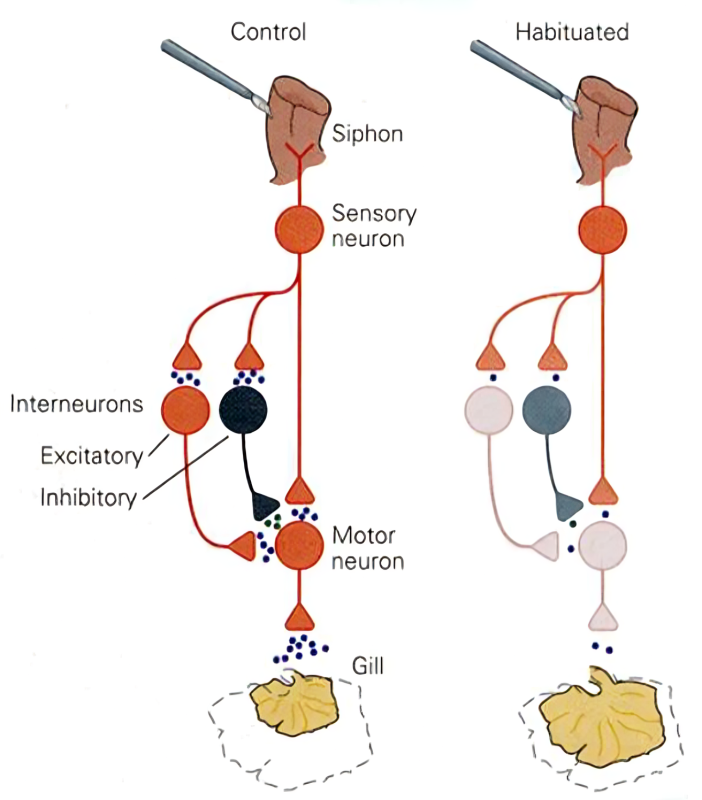
\includegraphics[width=0.9\linewidth]{./img/gill_habituation.png}
\end{minipage}



\section{Dopamine}

There is evidence that dopamine is involved in learning action-outcome associations.

\begin{description}
    \item[Striatal activity on unexpected events] \marginnote{Striatal activity on unexpected events}
        When an unexpected event happens, there is a change in the activity of the striatum.
        There is an increase in response when the feedback is positive and a decrease when negative.

        \begin{casestudy}[Microelectrodes in substantia nigra]
            \phantom{}\\
            \begin{minipage}{0.7\linewidth}
                The activity of the substantia nigra of patients with Parkinson's disease is measured during a probabilistic instrumental learning task.
                The task consists of repeatedly drawing a card from two decks, followed by positive or negative feedback depending on the deck.
            \end{minipage}
            \begin{minipage}{0.3\linewidth}
                \centering
                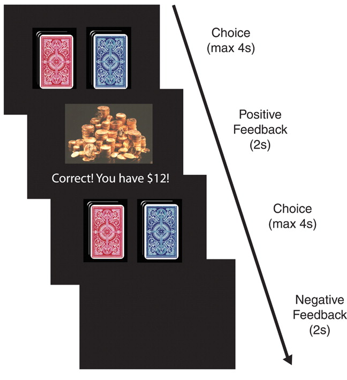
\includegraphics[width=0.95\linewidth]{./img/instrumental_dopamine_sn1.png}
            \end{minipage}

            The increase and decrease in striatal activity can be clearly seen when the feedback is unexpected.
            \begin{figure}[H]
                \centering
                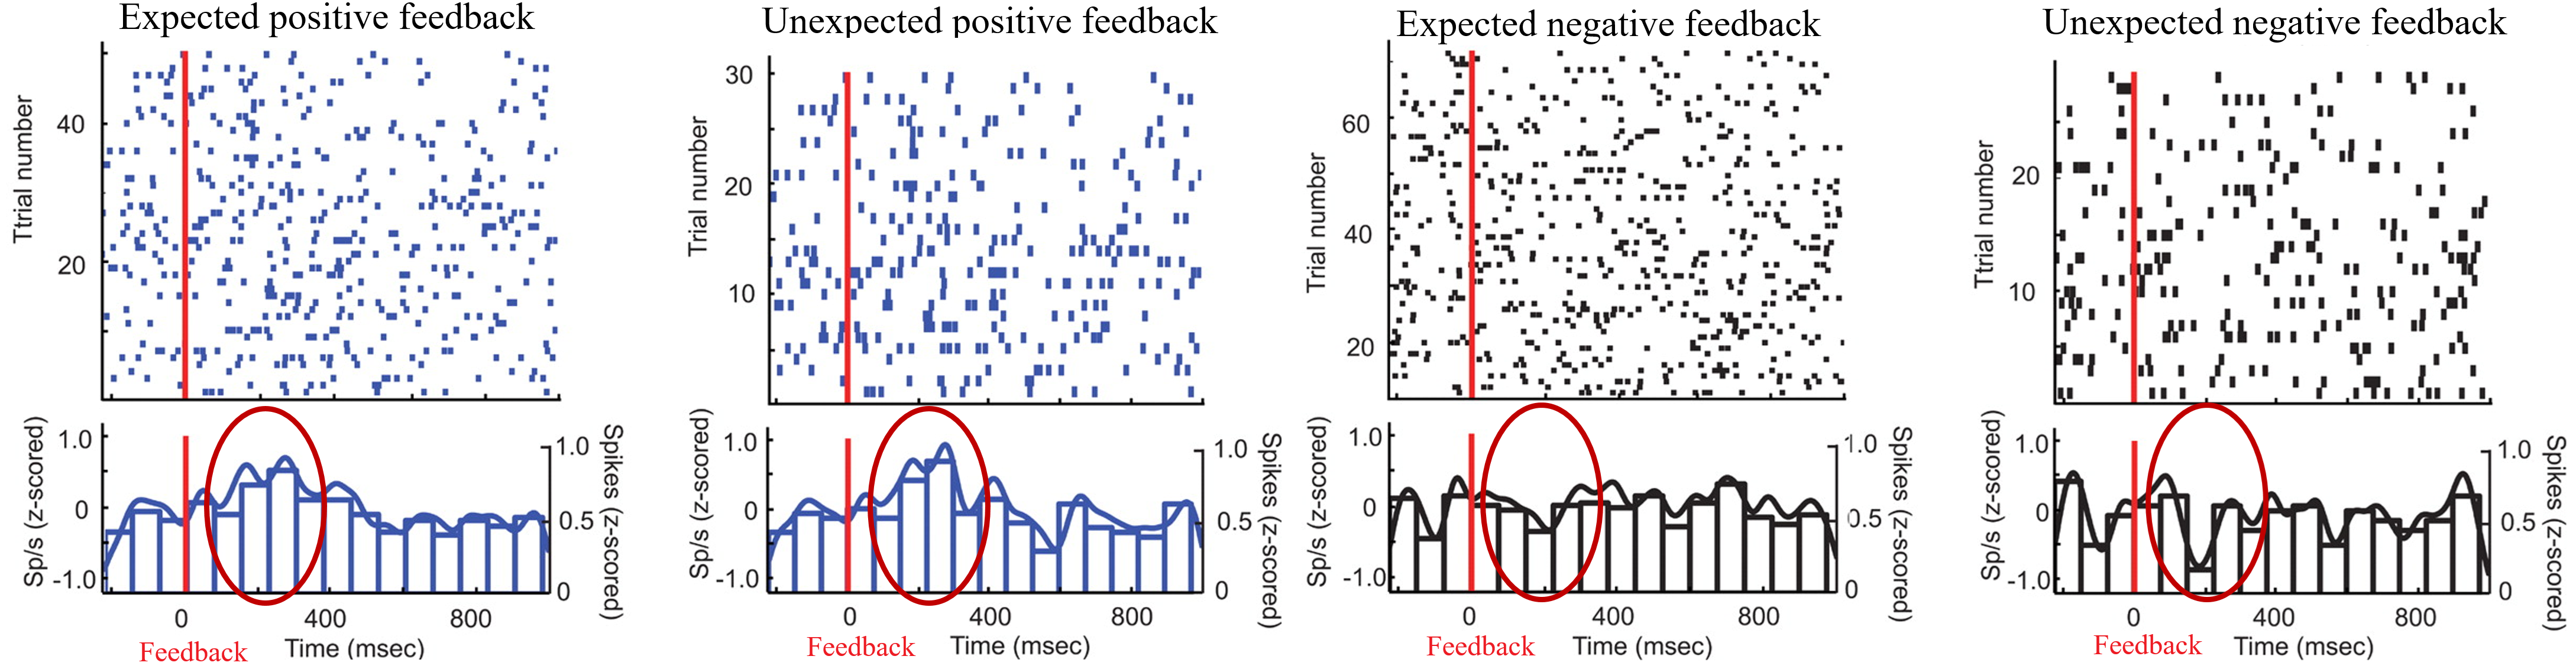
\includegraphics[width=\linewidth]{./img/instrumental_dopamine_sn2.png}
            \end{figure}
        \end{casestudy}

    \item[Dopamine effect on behavior] \marginnote{Dopamine effect on behavior}
        The amount of dopamine changes the learning behavior:
        \begin{itemize}
            \item Low levels of dopamine cause an impairment in learning from positive feedback.
                This happens because positive prediction errors cannot occur.
            
            \item High levels of dopamine cause an impairment in learning from negative feedback.
                This happens because negative prediction errors cannot occur.
        \end{itemize}

        \begin{casestudy}[Probabilistic selection task]
            This instrumental learning task has two phases:
            \begin{descriptionlist}
                \item[Learning]
                    There are three pairs of stimuli (symbols) and, at each trial, a pair is presented to the participant who selects one.
                    For each pair, a symbol has a higher probability of providing positive feedback while the other is more likely to be negative.
                    Moreover, the probabilities are different among the three pairs.

                    \begin{center}
                        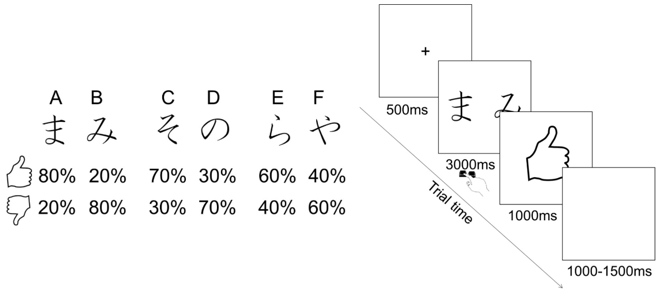
\includegraphics[width=0.55\linewidth]{./img/instrumental_dopamine_selection1.png}
                    \end{center}

                    Participants are required to learn by trial and error the stimulus in each pair that leads to a positive reward.
                    Note that learning could be accomplished by:
                    \begin{itemize}
                        \item Recognizing the more rewarding stimulus.
                        \item Recognizing the less rewarding stimulus.
                        \item Both.
                    \end{itemize}

                \item[Testing]
                    Aims to assess if participants learned to select positive feedback or avoid negative feedback.

                    The same task as above is repeated but all combinations of the stimuli among the three pairs are possible.
            \end{descriptionlist}

            Three groups of participants are considered for this experiment:
            \begin{enumerate}
                \item Those who took the cabergoline drug (dopamine antagonist).
                \item Those who took the haloperidol drug (dopamine agonist).
                \item Those who took a drug without effects (placebo).
            \end{enumerate}

            \begin{center}
                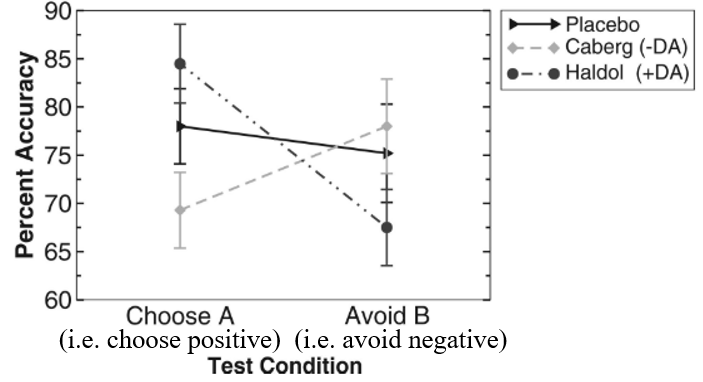
\includegraphics[width=0.55\linewidth]{./img/instrumental_dopamine_selection2.png}
            \end{center}

            Results show that:
            \begin{enumerate}
                \item Cabergoline inhibited positive feedback learning.
                \item Haloperidol enhanced positive feedback learning.
                \item Placebo learned positive and negative feedback equally.
            \end{enumerate}
        \end{casestudy}
        
        \begin{casestudy}
            It has been observed that:
            \begin{itemize}
                \item Reward prediction errors are correlated with activity in the left posterior putamen and left ventral striatum.
                \item Punishment prediction errors are correlated with activity in the right anterior insula.
            \end{itemize}

            \begin{center}
                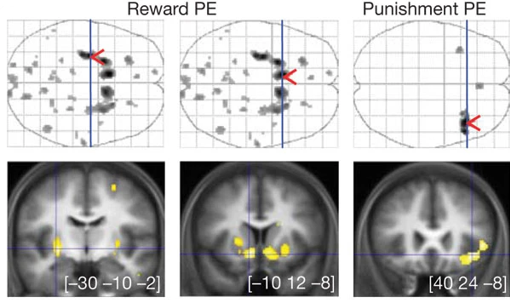
\includegraphics[width=0.5\linewidth]{./img/pe_location.png}
            \end{center}
        \end{casestudy}

    \item[Actor-critic model] \marginnote{Actor-critic model}
        Model to correlate Pavlovian and instrumental learning. 
        It is composed by:
        \begin{itemize}
            \item The cortex is responsible for representing the current state.
            \item The basal ganglia implement two computational models:
                \begin{descriptionlist}
                    \item[Critic] \marginnote{Critic}
                        Learns stimulus-outcome associations and is active in both Pavlovian and instrumental learning.
                        It might be implemented in the ventral striatum, the amygdala and the orbitofrontal cortex.
                
                    \item[Actor] \marginnote{Actor}
                        Learns stimulus-action associations and is only active during instrumental learning.
                        It might be implemented in the dorsal striatum.
                \end{descriptionlist}
        \end{itemize}
\end{description}

\begin{casestudy}[Food and cocaine]
    \phantom{}
    \begin{itemize}
        \item Food-induced dopamine response is modulated by the reward expectations that promote learning until the prediction matches the actual outcome.
        \item Cocaine-induced dopamine response causes a continuous increase in the predicted reward that
            will eventually surpass all other cues and bias decision-making towards cocaine.
    \end{itemize}
    \begin{center}
        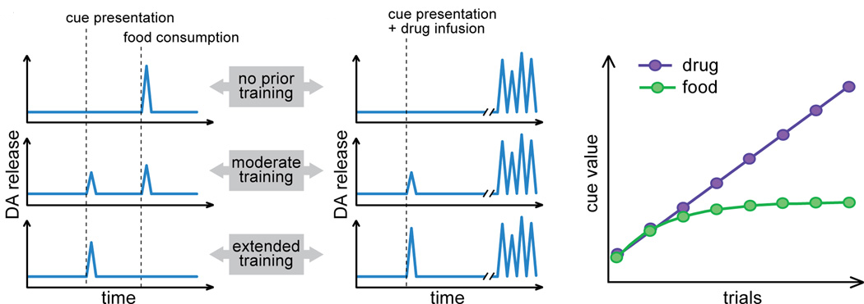
\includegraphics[width=0.8\linewidth]{./img/dopamine_food_cocaine.png}
    \end{center}
\end{casestudy}



\section{Learning strategies historical evolution}


% Instrumental learning can happen in two ways:
% \begin{descriptionlist}
%     \item[Cognitive map] \marginnote{Cognitive map}
%         Actions are taken based on the expected reward.
    
%     \item[Response strategy] \marginnote{Response strategy}
%         Actions are associated with particular stimuli.
% \end{descriptionlist}


\subsection{Generation 0}

There were two possible learning strategies:
\begin{descriptionlist}
    \item[Stimulus-response theory] \marginnote{Stimulus-response theory}
        Learning happens by creating stimulus-response associations.

        Learning does not happen if there is no reward.

    \item[Cognitive map / Field theory] \marginnote{Cognitive map / Field theory}
        A mental map is created and used to find the best action in a given state based on the expected reward.

        \begin{description}
            \item[Latent learning] \marginnote{Latent learning}
                Learning that is not shown behaviorally unless there is enough motivation.
        \end{description}
\end{descriptionlist}

\begin{casestudy}[Maze]
    An animal is put at the start of a maze where a reward is located in the west arm.
    After some training iterations, the animal is put at the other entrance:
    \begin{itemize}
        \item If it goes to the west arm, it learned to solve the maze using a cognitive map/place strategy.
        \item If it goes to the east arm, it learned to solve the maze using a stimulus-response strategy.
    \end{itemize}
    \begin{center}
        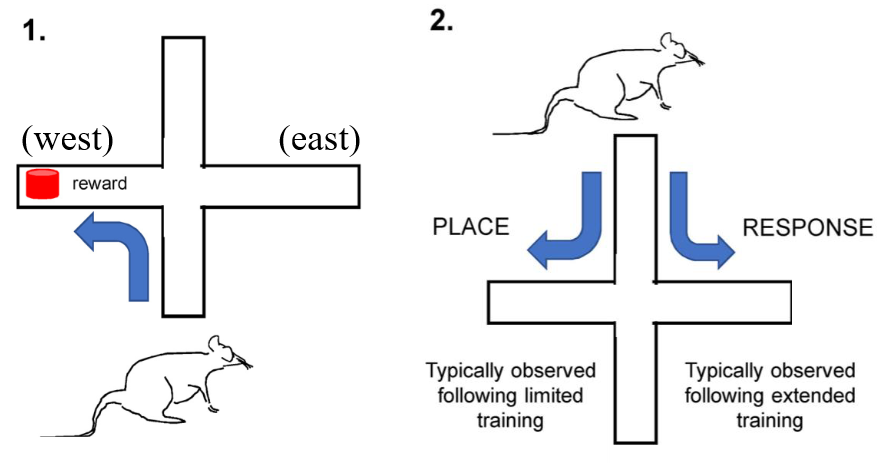
\includegraphics[width=0.55\linewidth]{./img/instrumental_maze.png}
    \end{center}

    It has been observed that rats start by learning a cognitive map (i.e. the environment is unknown).
    After enough training, they start relying on a response strategy (i.e. the environment is stable).
\end{casestudy}

\begin{casestudy}[Tolman's maze]
    Consider a maze with curtains and doors to prevent a long-distance perspective.
    \begin{center}
        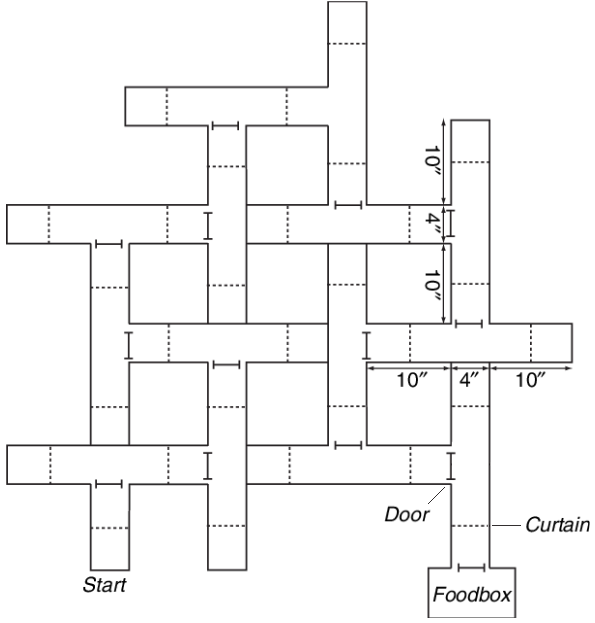
\includegraphics[width=0.35\linewidth]{./img/tolman_maze.png}
    \end{center}

    Two groups of hungry rats have been considered to solve the maze:
    \begin{descriptionlist}
        \item[Group 1] No reward for solving the maze.
        \item[Group 2] Reward for solving the maze.
    \end{descriptionlist}
    It has been shown that the second group completes the maze faster.
    \begin{center}
        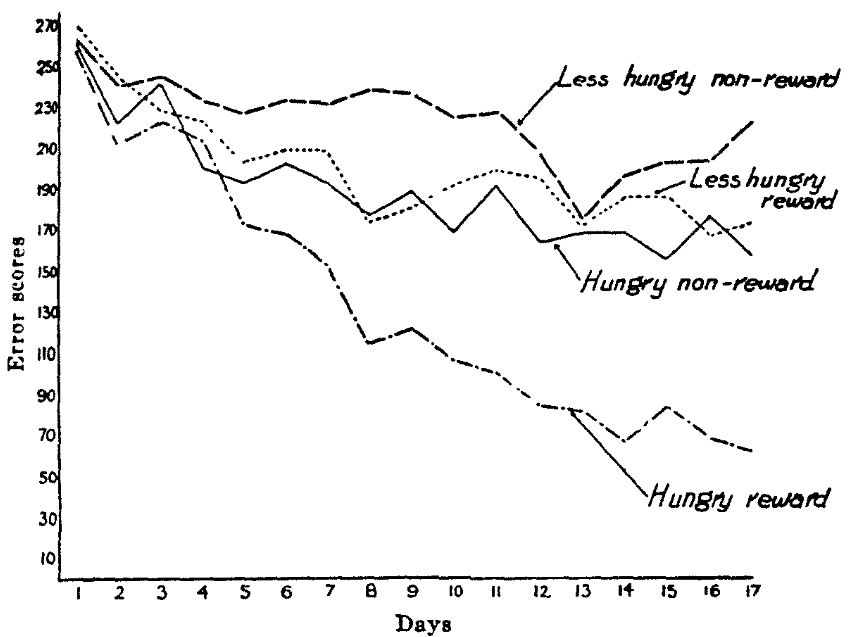
\includegraphics[width=0.45\linewidth]{./img/tolman_experiment1.png}
    \end{center}

    To show latent learning, three groups of hungry rats have been considered:
    \begin{descriptionlist}
        \item[Group 1] No reward for solving the maze.
        \item[Group 2] Reward for solving the maze.
        \item[Group 3] Reward for solving the maze starting from day 11.
    \end{descriptionlist}
    It has been shown that rats of the third group complete the maze faster as soon as they receive food.
    \begin{center}
        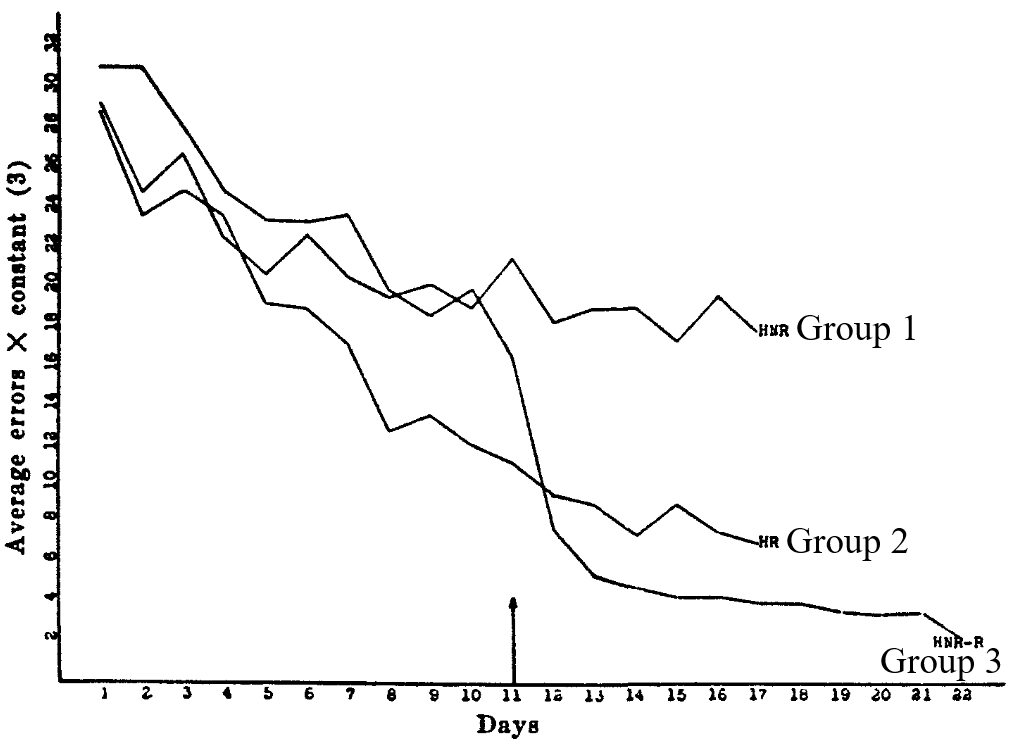
\includegraphics[width=0.45\linewidth]{./img/tolman_experiment2.png}
    \end{center}
\end{casestudy}


\subsection{Generation 1} 

Shifted from studying the spatial domain to a more general domain.
Based on two types of actions:
\begin{descriptionlist}
    \item[Goal-directed action] \marginnote{Goal-directed action}
        Actions made because a desired outcome is expected.
        An action is goal-directed if:
        \begin{itemize}
            \item There is knowledge of the relationship between action and consequences (response-outcome).
            \item The outcome is motivationally relevant.
        \end{itemize}

        Goal-directed behavior has the following properties:
        \begin{itemize}
            \item Involves active deliberation.
            \item Has a high computational cost.
            \item It is flexible to changes of the environmental contingency (i.e. stops if no reward occurs)
        \end{itemize}

        \begin{center}
            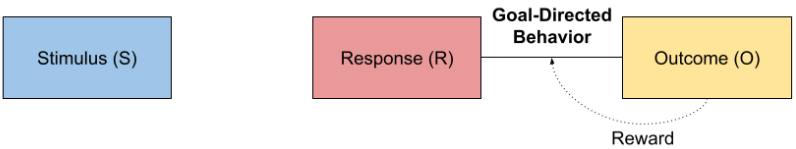
\includegraphics[width=0.65\linewidth]{./img/goal_directed_behavior.png}
        \end{center}

    \item[Habitual action] \marginnote{Habitual action}
        Actions made automatically just because they were rewarded in the past.
        They are not influenced by the current outcome even if it is undesired.

        Habitual behavior has the following properties:
        \begin{itemize}
            \item Does not require active deliberation.
            \item Has a low computational cost.
            \item It is inflexible to changes of the environmental contingency.
        \end{itemize}

        \begin{center}
            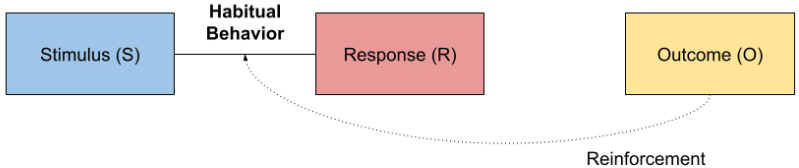
\includegraphics[width=0.65\linewidth]{./img/habitual_behavior.png}
        \end{center}

\end{descriptionlist} 

\begin{casestudy}[Goal-directed vs habitual behavior]
    The experiment is done in three steps:
    \begin{descriptionlist}
        \item[Training] 
            The animal undergoes instrumental learning (e.g. associate that by pressing a lever some food will be dropped).
        
        \item[Devaluation] 
            Manipulate the learned behavior by either:
            \begin{itemize}
                \item Devaluate the reinforcer.
                \item Degradate the contingency.
            \end{itemize}

        \item[Testing] 
            Repeat the training scenario without reward:
            \begin{itemize}
                \item If the action associated with a devaluated reinforcer is performed less, the behavior is goal-directed.
                \item If the frequency of the action is the same, the behavior is habitual.
            \end{itemize}
    \end{descriptionlist}

    \begin{remark}
        The training phase aims to instill a goal-directed behavior.
        On the other hand, if the animal is overtrained, it will learn a habitual behavior.
        The experiment can be done both ways.
    \end{remark}

    \begin{center}
        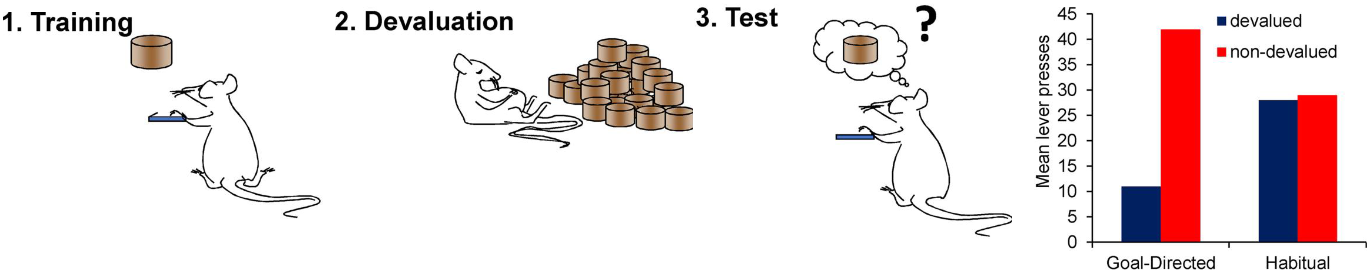
\includegraphics[width=0.85\linewidth]{./img/goal_directed_vs_habitual.png}
    \end{center}
\end{casestudy}

It has been hypothesized that the striatum might be the interface where rewards influence actions as: \marginnote{Striatum}
\begin{itemize}
    \item The basal ganglia are involved in the selection of actions.
    \item The SNc affects the plasticity of the striatum through the release of dopamine.
\end{itemize}

Moreover, different sections of the striatum are responsible for different types of behavior:
\begin{descriptionlist}
    \item[Dorsomedial striatum] Supports goal-directed behavior.
    \item[Dorsolateral striatum] Supports habitual behavior.
\end{descriptionlist}
This also hints that goal-directed and habitual behaviors act simultaneously and competitively (see \hyperref[sec:instrumental_gen3]{Generation 3}).


\subsection{Generation 2} 

Studied goal-directed and habitual behavior in humans.

\begin{description}
    \item[Functional magnetic resonance imaging (fRMI)] \marginnote{Functional magnetic resonance imaging (fRMI)}
        Measures the ratio of oxygenated to deoxygenated hemoglobin molecules in the brain.
        It allows to indirectly measure the neuronal activity of the brain on a high spatial resolution (i.e. allows to see where things happen but not when).
\end{description}

\begin{casestudy}[Goal-directed behavior in humans]
    Candidates are trained to select between two fractals of which 
    one leads to a reward with a high probability and the other with a low probability.
    The possible rewards are chocolate, tomato juice and orange juice (used as a control outcome).

    \begin{figure}[H]
        \centering
        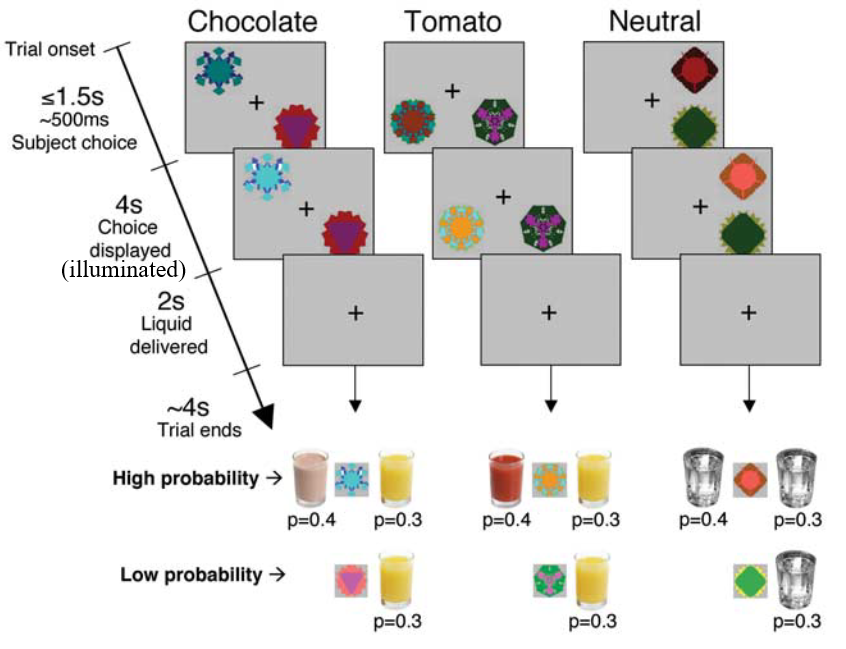
\includegraphics[width=0.45\linewidth]{./img/human_goal_directed_experiment.png}
        \caption{
            Structure of the task. The high probability choice leads to the primary reward (chocolate or tomato juice) with probability $0.4$, 
            to the control reward (orange juice) with probability $0.3$ and to nothing with probability $0.3$.
            The low probability choice leads to the control reward with probability $0.3$ and nothing in the other cases.
            The neutral case leads to an empty glass or nothing.
        }
    \end{figure}

    After training, one of the primary rewards is devalued through selective satiation and the other is labeled as the valued outcome.
    Then, the training task is repeated.
    \begin{figure}[H]
        \centering
        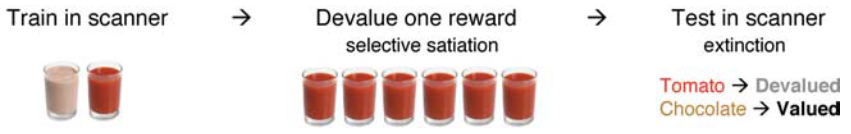
\includegraphics[width=0.55\linewidth]{./img/human_goal_directed_experiment2.png}
        \caption{
            Steps of the experiment. In this figure, the devalued reward is the tomato juice.        
        }
    \end{figure}

    Behavioral results show that:
    \begin{itemize}
        \item During training, candidates favored the high-probability actions associated with chocolate and tomato juice.
            On the other hand, choices for the neutral condition were evenly distributed.
        \item The pleasantness rating for the devalued reward lowered after devaluation while the valued reward remained higher.
        \item During testing, candidates reduced their choice of the high-probability action associated with the devalued reward.
    \end{itemize}
    \begin{figure}[H]
        \centering
        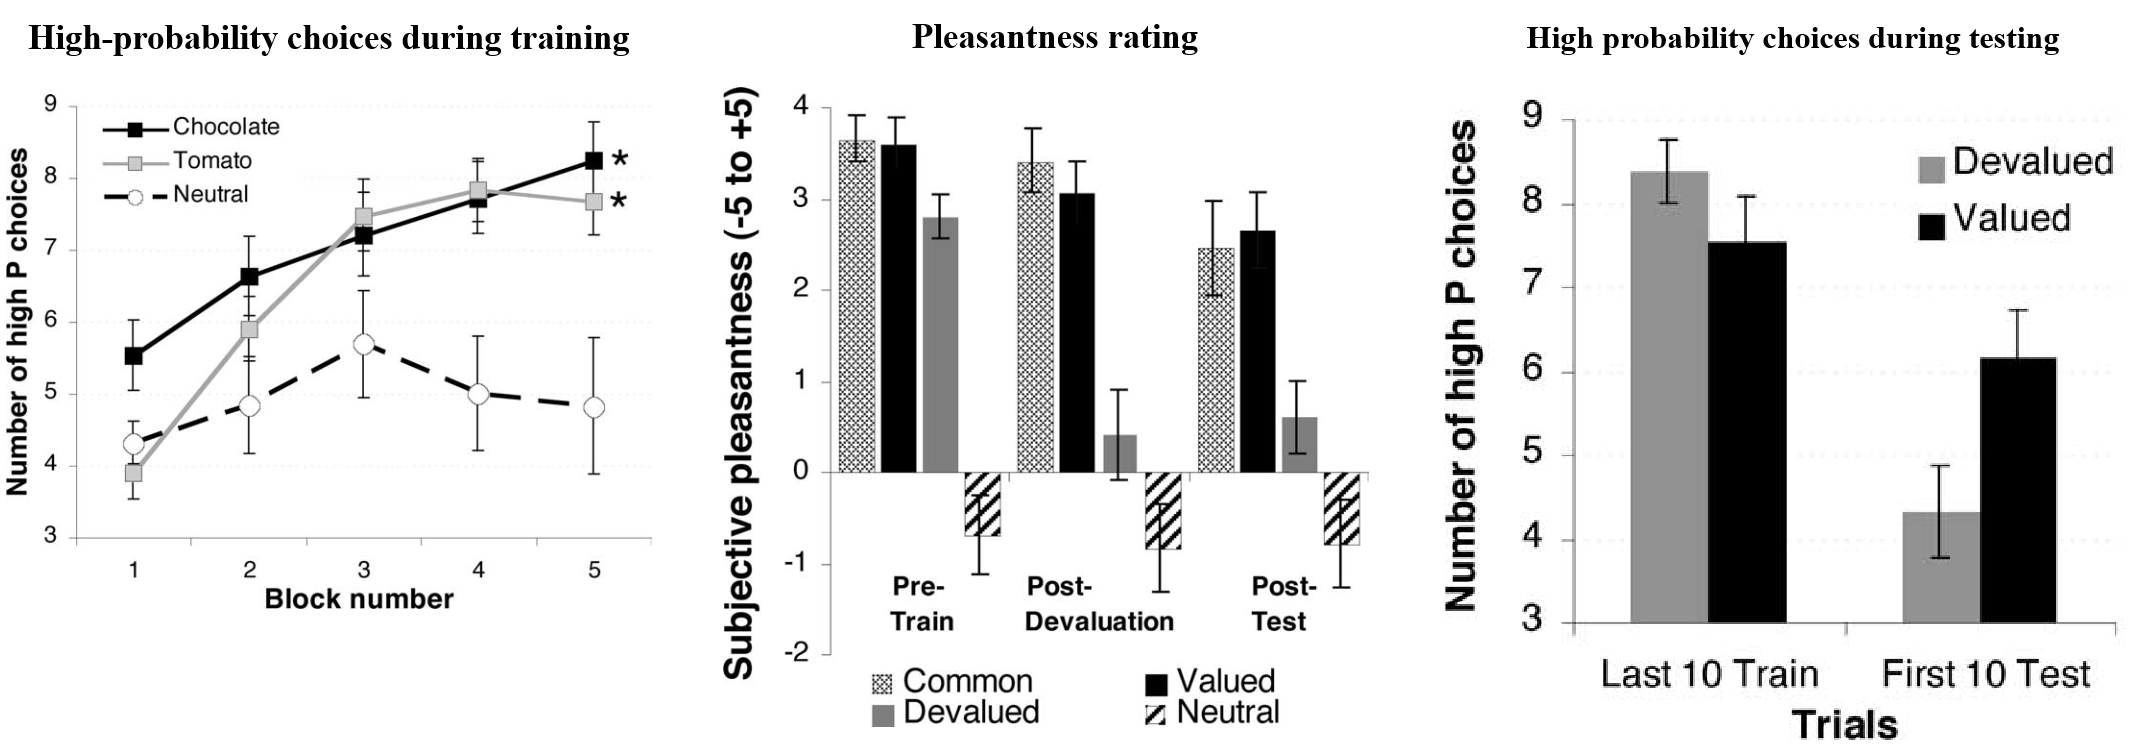
\includegraphics[width=0.9\linewidth]{./img/human_goal_directed_experiment3.png}
    \end{figure}

    During both training and testing, the fRMIs of the candidates were taken.
    Neural results show that the \textbf{medial orbitofrontal cortex }has a significant modulation in its activity during instrumental action selection
    depending on the value of the associated outcome.
    \begin{figure}[H]
        \centering
        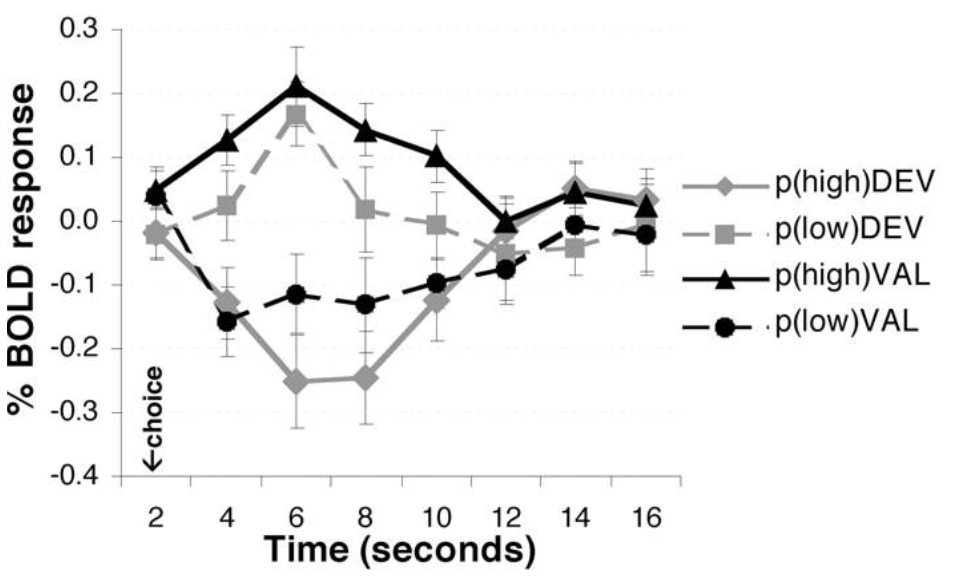
\includegraphics[width=0.4\linewidth]{./img/human_goal_directed_experiment4.png}
    \end{figure}
\end{casestudy}

\begin{casestudy}[Habitual behavior in humans]
    Candidates are presented, at each round of the trial, with a fractal image and a schematic indicating which button to press.
    The button can be pressed an arbitrary number of times and, at each press, on the screen appears:
    \begin{itemize}
        \item A gray circle (no reward).
        \item The image of an M\&M's {\tiny ©} or Frito {\tiny ©} (reward) with probability $0.1$. 
            To each fractal, only a type of reward can appear.
    \end{itemize} 
    \begin{figure}[H]
        \centering
        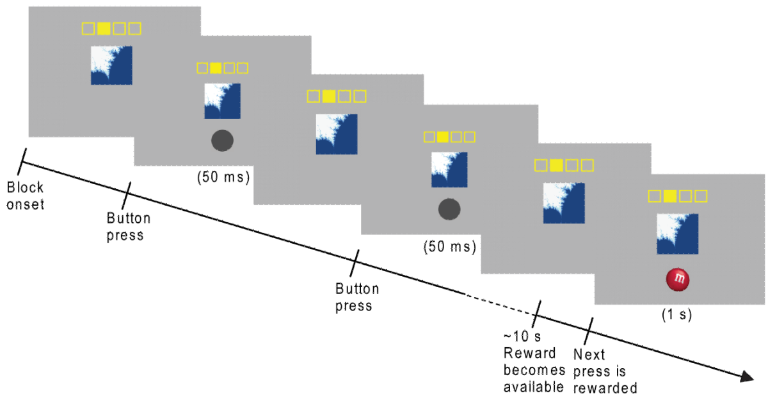
\includegraphics[width=0.6\linewidth]{./img/human_habitual_experiment.png}
    \end{figure}

    After training, one of the food rewards is devalued through selective satiation.
    Then, during testing, the same training task with the same stimulus-response-outcome is repeated without a reward.

    Two groups have been considered:
    \begin{descriptionlist}
        \item[1-day group] with little training.
        \item[3-day group] with extensive training.
    \end{descriptionlist}

    Behavioral results show that:
    \begin{itemize}
        \item Before devaluation, there were no significant differences between the responses of the two groups independently of the type of food.
        \item During testing, the 1-day group showed a goal-directed behavior while the 3-day group showed a habitual behavior.
    \end{itemize}
    \begin{figure}[H]
        \centering
        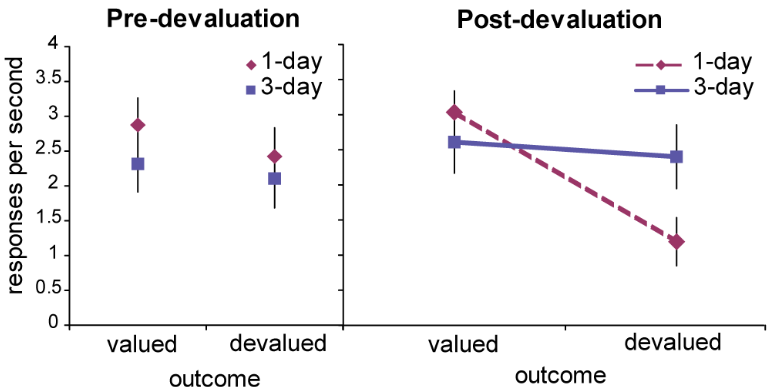
\includegraphics[width=0.55\linewidth]{./img/human_habitual_experiment2.png}
    \end{figure}

    During both training and testing, the fRMIs of the candidates were taken.
    Neural results show that, in the 3-day group, the \textbf{dorsolateral striatum} had significant activity.
\end{casestudy}


\subsection{Generation 3} \label{sec:instrumental_gen3}

Formalized goal-directed and habitual actions:

\begin{descriptionlist}
    \item[Model-based] (Goal-directed) \marginnote{Model-based}
        Use a model to predict the consequences of actions in terms of future states and expected rewards from future states.
    
        When the environment changes, the agent can update its policy of future states without the need to actually be in those states.

    \item[Model-free] (Habitual) \marginnote{Model-free}
        Select actions based on the stored state-action pairs learned over many trials.

        When the environment changes, the agent has to move into the new states and experience them.

    \item[Hybrid model] \marginnote{Hybrid model}
        Integrated computational and neural architecture where 
        model-based and model-free systems act simultaneously and competitively.

        This is the currently favored model for behavior.
\end{descriptionlist}


\begin{casestudy}[Latent learning in humans]
    The experiment consists of a sequential two-choice Markov decision task in which candidates navigate a binary decision tree.

    Each state contains a fractal image and
    candidates can choose to move to the left or right branch, each of which will lead with probability $0.7/0.3$ to one of the two subsequent states.
    When a leaf is reached, a monetary reward (0\textcentoldstyle, 10\textcentoldstyle\, or 25\textcentoldstyle) is delivered.
    \begin{figure}[H]
        \centering
        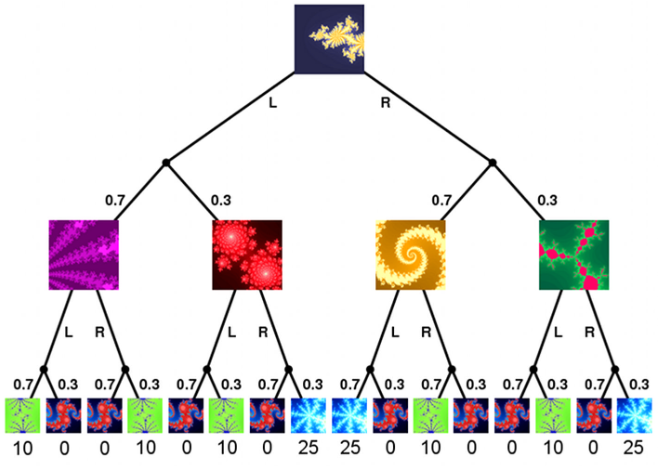
\includegraphics[width=0.4\linewidth]{./img/human_latent_experiment.png}
    \end{figure}

    \begin{minipage}{0.58\linewidth}
        The experiment is divided into two sessions:
        \begin{descriptionlist}
            \item[First session]
                Candidates choices are fixed but they can learn the transition probabilities.
    
            \item[Before second session]
                Candidates are presented with the association between fractal and reward.
    
            \item[Second session]
                Candidates are free to choose their actions at each state.
        \end{descriptionlist}
    \end{minipage}
    \begin{minipage}{0.4\linewidth}
        \centering
        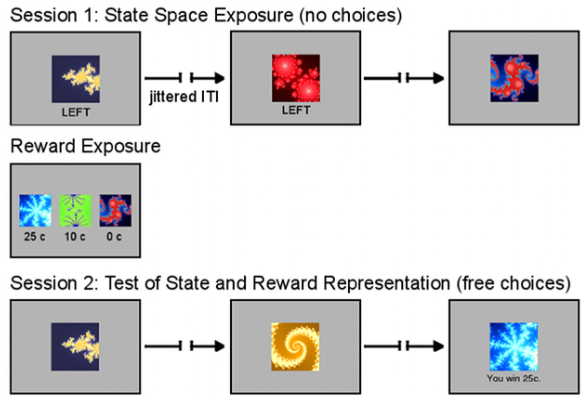
\includegraphics[width=0.95\linewidth]{./img/human_latent_experiment2.png}
    \end{minipage}\\[1em]

    \begin{minipage}{0.7\linewidth}
        Behavioral results show that the majority of the candidates are able to make the optimal choice.
        This indicates that their behavior cannot be explained using a model-free learning theory (as learning only happens with a reward).
        A hybrid model has been proposed to model the candidates' behavior. It includes:
        \begin{descriptionlist}
            \item[Reward prediction error] Associated to model-free learning.
            \item[State prediction error] Associated to model-based learning.
        \end{descriptionlist}
    \end{minipage}
    \begin{minipage}{0.3\linewidth}
        \centering
        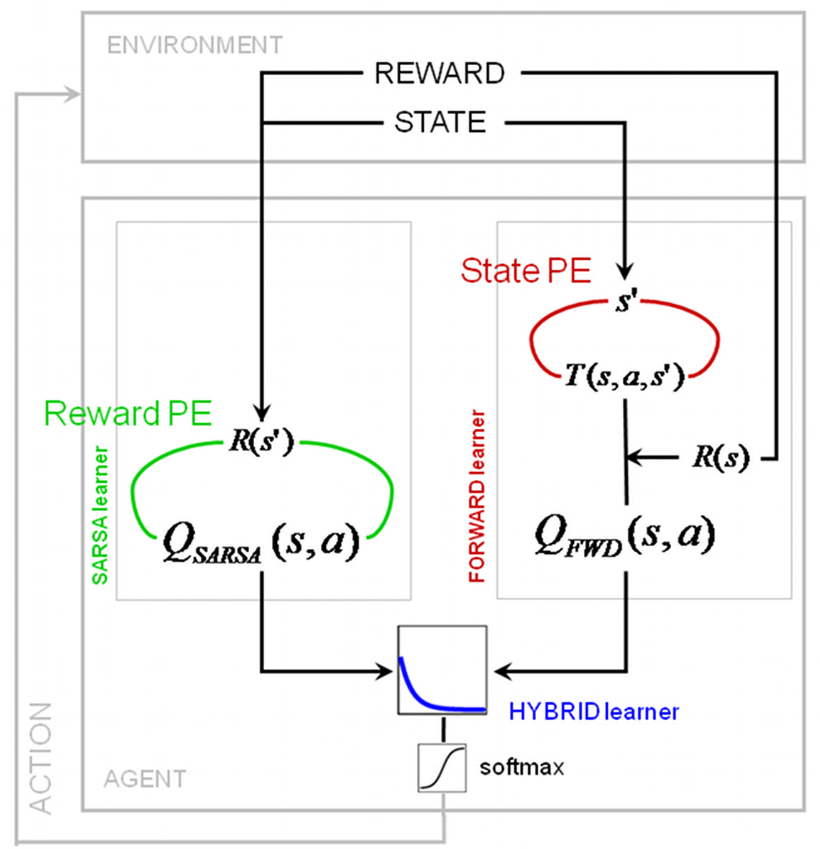
\includegraphics[width=\linewidth]{./img/human_latent_experiment3.png}
    \end{minipage}\\[1em]

    On a neuronal level, fRMIs show that:
    \begin{itemize}
        \item State prediction error activates the \textbf{intraparietal sulcus} and the \textbf{lateral prefrontal cortex}.
        \item Reward prediction error activates the \textbf{ventral striatum}.
    \end{itemize}
    \begin{figure}[H]
        \centering
        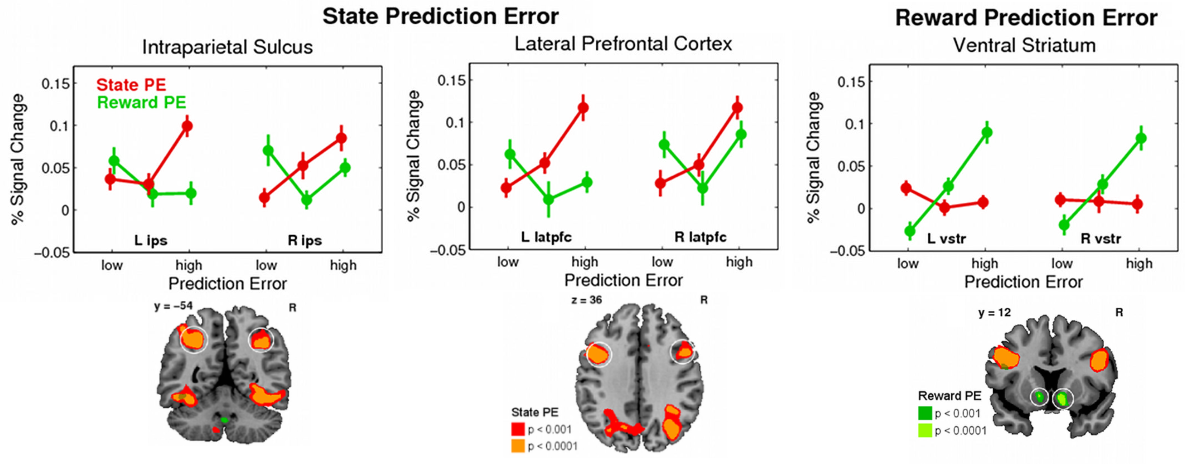
\includegraphics[width=0.75\linewidth]{./img/human_latent_experiment4.png}
    \end{figure}
\end{casestudy}

\begin{casestudy}[Model-free vs model-based in humans]
    Consider a Markov decision task that works as follows:
    \begin{itemize}
        \item In the first stage, candidates have to choose between two fractal images, 
            each leading to one of the two subsequent states with probability $0.7$ (common) and $0.3$ (rare).
        \item In the second stage, candidates have to choose between two fractal images, 
            each of which will lead to a monetary reward with a certain independent probability.
        \item The probability of receiving the reward changes stochastically during the trials.
    \end{itemize}
    \begin{figure}[H]
        \centering
        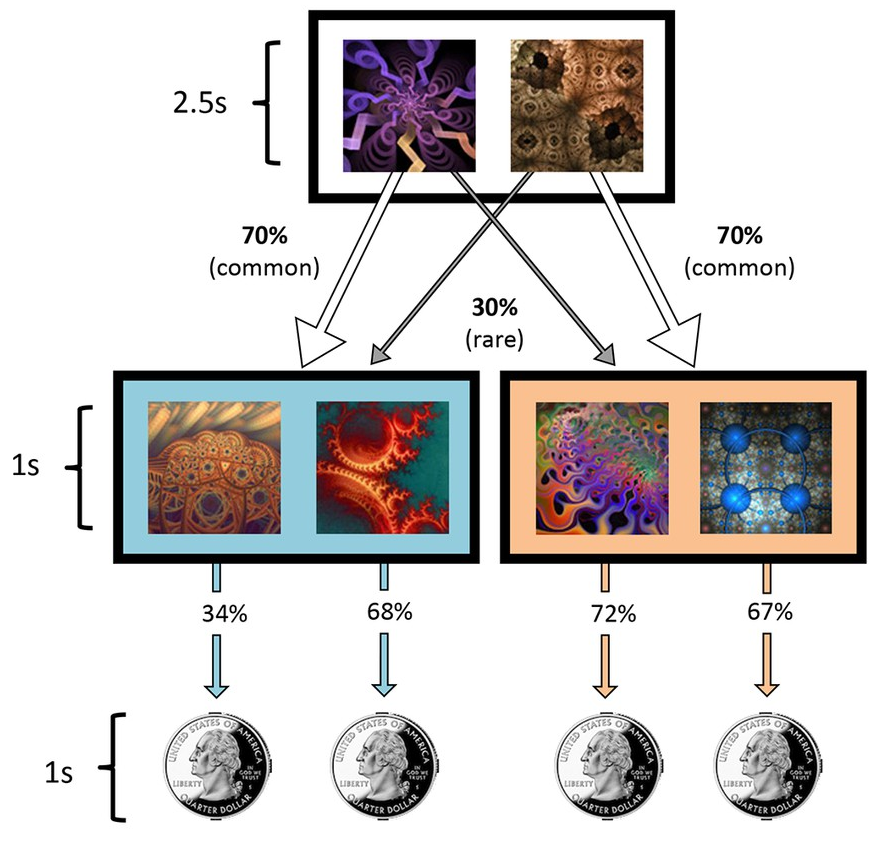
\includegraphics[width=0.35\linewidth]{./img/model_free_based_theoretical.png}
    \end{figure}

    It is expected that:
    \begin{descriptionlist}
        \item[Model-free agents] 
            Ignore the transition structure and prefer to repeat actions that lead to a reward in the past.

        \item[Model-based agents] 
            Respect the transition structure and modify their policies depending on the outcome.

            They are more likely to repeat an action following a rewarding trial only if that transition is common.
    \end{descriptionlist}

    Despite that, the actual results on human candidates show that a hybrid model is more suited to explain human behavior.
    \begin{figure}[H]
        \centering
        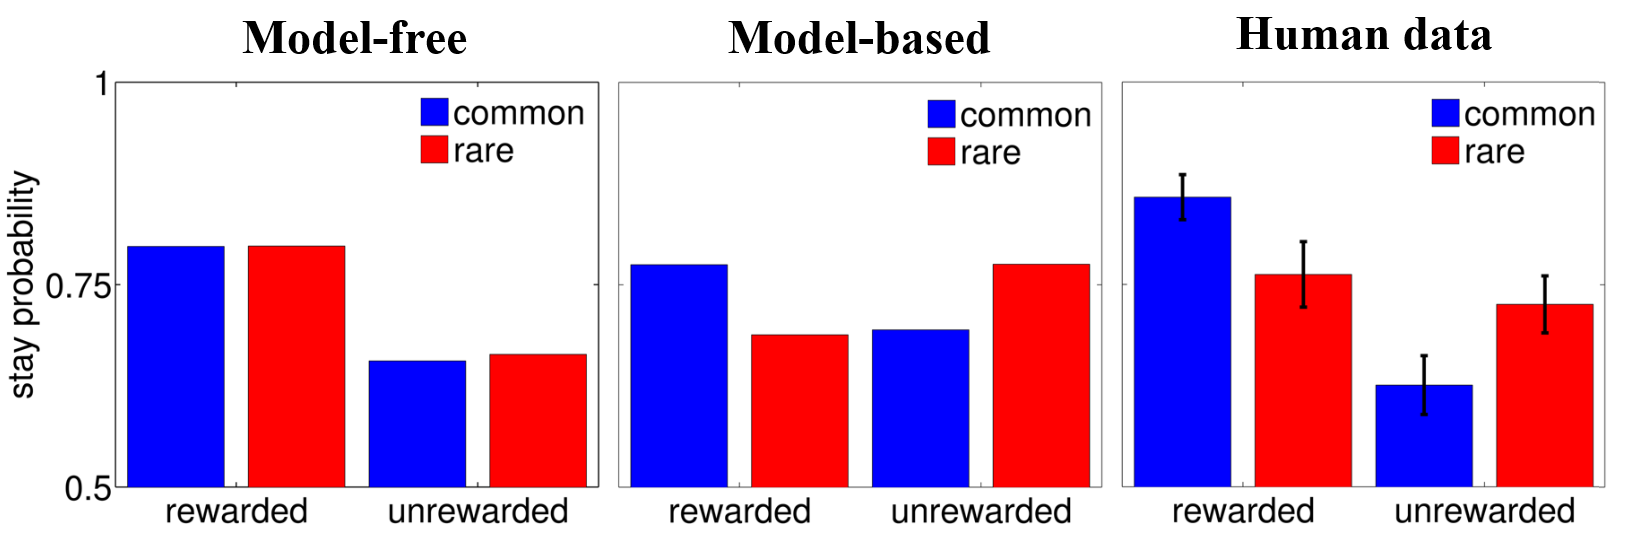
\includegraphics[width=0.6\linewidth]{./img/human_hybrid_model.png}
    \end{figure}

    % \begin{figure}[H]
    %     \centering
    %     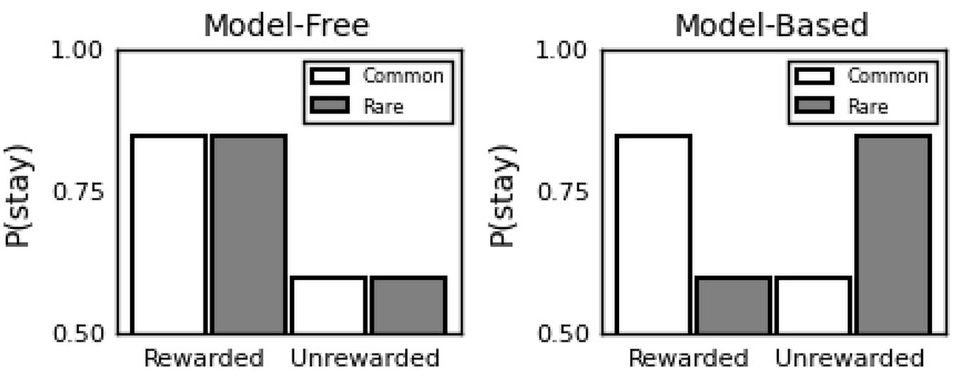
\includegraphics[width=0.5\linewidth]{./img/model_free_based_theoretical2.png}
    % \end{figure}

    Neural results from fRMIs also show that the activity in the \textbf{striatum} increases for both model-based and model-free prediction errors.
\end{casestudy}
